\section{Evaluation}
\label{sec:evaluation}
% We evaluate \OurSys using different types of traffic to measure its improvement
% to application-level behaviour in the presence of lossy links.

We evaluate \OurSys with microbenchmarks and network simulation to answer these questions:
\begin{itemize}

\item What are the resource requirements for \OurSys with different levels of 
error correction?

\item How much does \OurSys improve application throughput across lossy links?

%\item What benefit can \OurSys have to networks at large?
\end{itemize}

\subsection{Setup}
\begin{figure}
  \centering
  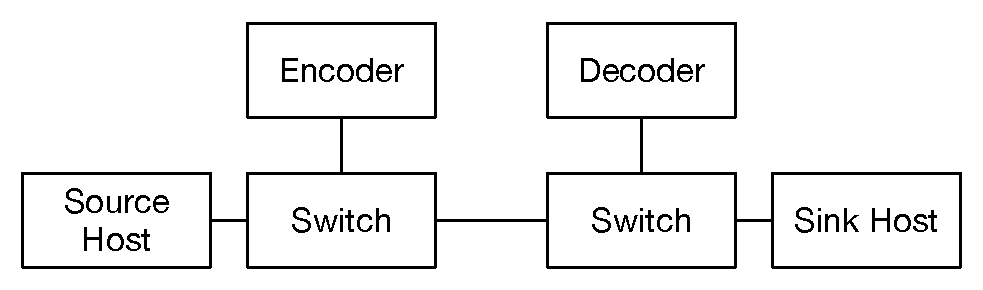
\includegraphics[width=0.3\paperwidth]{exp_topo.pdf}
  \caption{\label{fig:exp_topo} Testbed topology for benchmarks.}
\end{figure}

Figure~\ref{fig:exp_topo} depicts the testbed we used to benchmark \OurSys.
The two traffic generation hosts are each connected to different \OurSys
enabled switches, which are themselves connected by a 10 GbE link. The
switches are Wedge BF32-100X's with P4 programmable forwarding engines. We
evaluate three possible deployment models for \OurSys: an FPGA external to
the switch; a software implementation running on the switch CPU; and an ASIC  
implementation integrated into the switch forwarding engine. 

\subsection{\OurSys models}
\subsubsection{Behavioral model}
Figure~\ref{fig:app_tput} shows iperf throughput in the testbed as link quality
decreases, using the behavioral model of \OurSys.
To benchmark the ASIC implementation, we use a behavioral model. Instead  of
dropping packets, the switches tag packets to be dropped in their  egress
pipelines. The receiving switch recirculates all the data packets in a block 
until it either counts K distinct packets from that block, i.e., the number of packets 
required to decode, or a single packet from a subsequent block. If the counter 
reached K, \OurSys models a successful decode by stripping any tags from the 
data packets in the block and forwarding them on. On the other hand, if 
a packet from the next block arrives before the decode is complete, \OurSys 
models a failed decode by simply dropping all the packets from the current 
block and moving on to the next one. 


\subsubsection{Event-based simulation}
Figure/Table~\ref{tab:simulation} shows something about the overall benefit of \OurSys from a network-wide perspective, based on an ns-3 event-driven simulation.
This model has better fidelity than the previous model, but is not run on real hardware. This also means we can simulate larger networks. Here we present data for experiments that are comparable to the setups used in the other evaluations.


\subsection{Encoder Microbenchmarks}
Here we evaluate the implementation directly, not using a model.
Latency and throughput graphs for experiments involving different loss rates, and the encoder working on the CPU and FPGA.
Note: we have not optimised the CPU implementation.


\subsection{FPGA resource consumption}
Table~\ref{tab:microbenchmarks} shows the resource requirements for the FPGA implementations of
\OurSys with different H and K parameters.
%CPU cycles for the software
%implementation are measured using Linux performance counters and averaged over
%X packets,
FPGA requirements are obtained from the Xilinx compiler, and the
timing statistics are measured using ingress and egress timestamps on
the switch.

\begin{figure}
  \centering
  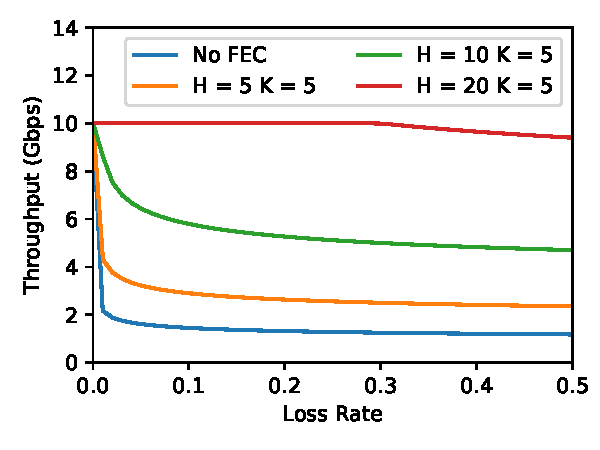
\includegraphics[width=0.3\paperwidth]{fake_tput.pdf}
  \caption{\label{fig:app_tput} Application throughput.}
\end{figure}

\begin{table}
% \footnotesize
\begin{center}
\small
% \resizebox{\linewidth}{!}{
\begin{tabular}{ l l l l l } 
\toprule
(H, K) & (5,3) & (10,3) & (20,3) & (40,3) \\
\midrule
\emph{Software} & & & & \\
\cmidrule{1-1}
Cycles & & & & \\
Processing Time (ns) & & & & \\
\midrule
\emph{FPGA} & & & & \\
\cmidrule{1-1}
??? & & & & \\
??? & & & & \\
Processing Time (ns) & & & & \\
\bottomrule

\end{tabular}
% }
\caption{Resource requirements for FPGA and CPU implementations of \OurSys with different configurations.}
\label{tab:microbenchmarks}
\end{center}
\end{table}


%We run \OurSys in 3 configurations: outside the switch, on the switch, and in the switch.
%Time how quickly \OurSys reacts to failing links.
